\section{Projektorganisering}
\subsection{Generell struktur}
Generellt sett är projektet strukturerat genom att teamet utveckla en produkt till kunden och använder sig av
handledaren för generella frågor kring projektstruktur samt för att se till att ett stadigt tempo upphålls.
Kommunikationen med handledaren går via teamledaren och kommunikation med kund sker via analysansvarig. Dessa roller
beskrivs vidare under \textit{Roller}. Teamet har också skrivit ett gruppkontrakt\cite{bib-gruppkontrakt} som alla gått med på att följa.
\begin{figure}[t]
    \centering
    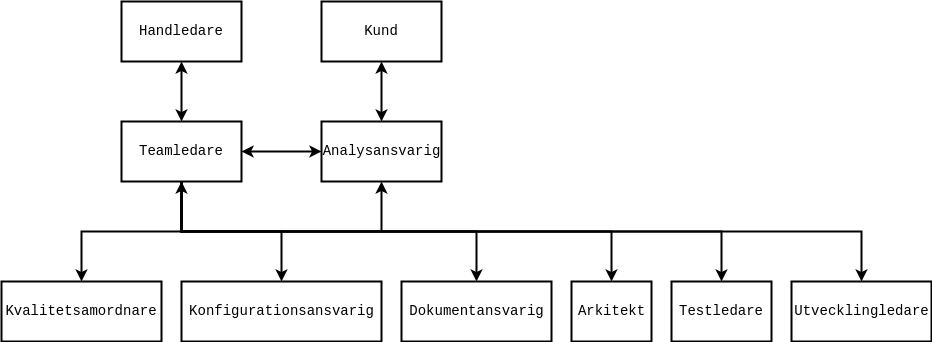
\includegraphics[scale=0.4]{struktur}
    \caption{Projektstruktur}
    \label{fig:struktur}
\end{figure}\\



\subsection{Roller}
\begin{center}
    \begin{tabular}{| l | l |}
        \hline
        \textbf{Namn} & \textbf{Roll} \\
        \hline
        \centering Alexander Wilkens & Teamledare\\
        \hline
        \centering Joel Almqvist & Kvalitetssamordnare\\
        \hline
        \centering Tim Håkansson & Dokumentansvarig\\
        \hline
        \centering Joel Oskarsson & Arkitekt\\
        \hline
        \centering Lieth Wahid & Utvecklingsledare\\
        \hline
        \centering Axel Löjdquist & Analysansvarig\\
        \hline
        \centering David Kjellström & Testledare\\
        \hline
        \centering Björn Detterfelt & Konfigurationsansvarig\\
        \hline
    \end{tabular}
\end{center}
\subsubsection*{Teamledare}
Teamledaren ska se till att samtliga processer som ska utföras i projektets gång följs. Denna person representerar också teamet utåt och har kontakt med handledaren. Om det behövs har teamledaren sista ordet.

\subsubsection*{Kvalitetssamordnare}
Kvalitetssamordnaren ansvarar för arbetsprocesser som ska hålla kvaliten av projektet på en hög nivå. Gör en budget av vad kvalitet får kosta och ansvarar för kvalitetsplanen.

\subsubsection*{Dokumentansvarig}
Dokumentansvarig ser till att ansvara för samtliga dokument som teamet ska producera. Även ansvarig för gruppens logotyp och dokumentmallar.

\subsubsection*{Arkitekt}
Arkitekten ansvarar för att arkitekturen av den tekniska delen av projektet. Gör övergripande teknikval och har det sista ordet på tekniska beslut.

\subsubsection*{Utvecklingsledare}
Utvecklingsledaren ansvarar för den mer detaljerade designen av den tekniska produkten. Leder utvecklingsarbetet och ser till att resten av teamet har något att arbeta med.

\subsubsection*{Analysansvarig}
Analysansvarig ansvarar för majoriteten av kundkontakt och jobbar ständigt med att ta reda på kundens verkliga behov. Har huvudansvar för kravspecifikationen.

\subsubsection*{Testledare}
Testledaren beslutar systemets status genom att arbeta tillsammans med kvalitetssamordnaren för att testa så systemet uppnår kraven. Skriver testplan och testrapport.

\subsubsection*{Konfigurationsansvarig}
Konfigurationsansvarig ansvarar för generell versionshantering i projektet. Arbetar mycket med utvecklingledaren och dokumentansvarig för att bestämma vilka arbetsprodukter som ska ingå i en utgåva(release).


\subsection{Kunskap och erfarenheter}
Alla projektmedlemmar har läst flera år på civilingenjörsprogrammet i datateknik respektive mjukvaruteknik. Teamet förväntas ha kunskaper och erfarenheter från de tidigare kurser och projekt som utförs i utbildning. Extra fokus ligger på de kurser som studiehandboken listar som förkunskapskrav till TDDD96\cite{bib-tddd96}.


\subsection{Utbildning}
Mycket av den kunskap som teamet kommer behöva ha för att utföra projektet kommer införskaffas via självstudier. Innan implementationsdelen av projekt drar igång kommer teamet också få chans att ha en genomgång av Cybercoms API och backend.
\\
Varje projektmedlem är också ansvarig för att sätta sig in i eventuella ramverk och andra tekniker som ska användas i den kommande sprinten.

\subsection{Kommunikation och rapportering}
Teamet ska under projektets gång producera veckorapporter som ska lämnas in till handledare senast måndag varje vecka. Veckorrapporten beskriver vad teamet jobbat med under den senaste veckan, vad de ska jobba med i veckan som kommer samt eventuella risker som finns som kan på något sätt hindra projektet. Innan rapporten skickas in ska teamet ha möte för att bestämma innehållet och diskutera arbete inför veckan. En uppdaterad tidsrapport bifogas också.\\
\\
Kommunikationen i teamet sker antingen i person eller via Slack. Kommunikation mellan teamet och handledaren sker via mail genom teamledaren. Kundkommunikation sker antingen i Slack eller via mail genom analysansvarig.

\pagebreak
